\chapter{Operational Information}

\section{Class Masking}

To classify the picture as closely as possible to the desired result, it was necessary to review the details of the image for any features that could be extracted at an elementary level. The elementary level in this case is the raw image data available through individual pixel values. The support vector machine implementation in Matlab allowed for as many classification parameters to be passed for generating the classification structure. 

\begin{figure}[ht]
    \centering
    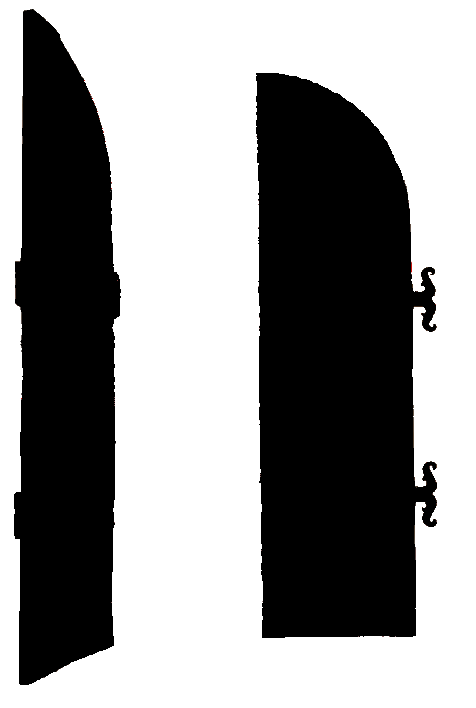
\includegraphics[height=3in]{00_classmask}
    \caption{Classification Mask used to determine class of training points}
    \label{fig:00_classmask}
\end{figure}

When using the class mask, as seen in \ref{fig:00_classmask}, it was necessary to generate a set of points to apply to the mask which maximized the positive effect on the support vector machine while reducing the requirement for an overly high number of required points. 

As explained by Dr. Haykin, the support vector machine internally tries to maximize the distance between the points it is currently training against and the desired hyperplane\citep{SH_hyperplane0}. Randomly generating points from the entire images with no concern for position doesn't benefit the areas in the image where the distinction between both classes is quite complex. 

\section{Point Generation and Pooling}

A method for promoting certain parts of the image while also allowing for automation of point generation is shown below. By applying a Gaussian blur filter to the previous hard-edged mask, a new mask where the point densities increase relative to the distance to the mask boundary is generated.

\begin{figure}[p]
    \centering
    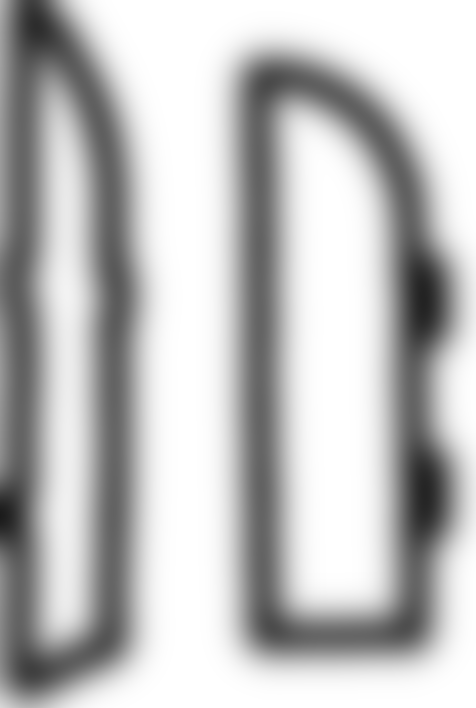
\includegraphics[height=3in]{01_densitymask}
    \caption{Mask relating desired point density to position}
    \label{fig:01_densitymask}
\end{figure}

The training point generator works by sampling points through probability specified by the pixel values on this density mask. Visually the colormap, as shown in \ref{fig:02_densitymask3D}, is an example in which the points will be more likely to be generated from. For small training sizes, there is no guarantee that points will exist from those levels in the produced training set as the pool itself is sampled and culled to bring forth the final training set.

\begin{figure}[p]
    \centering
    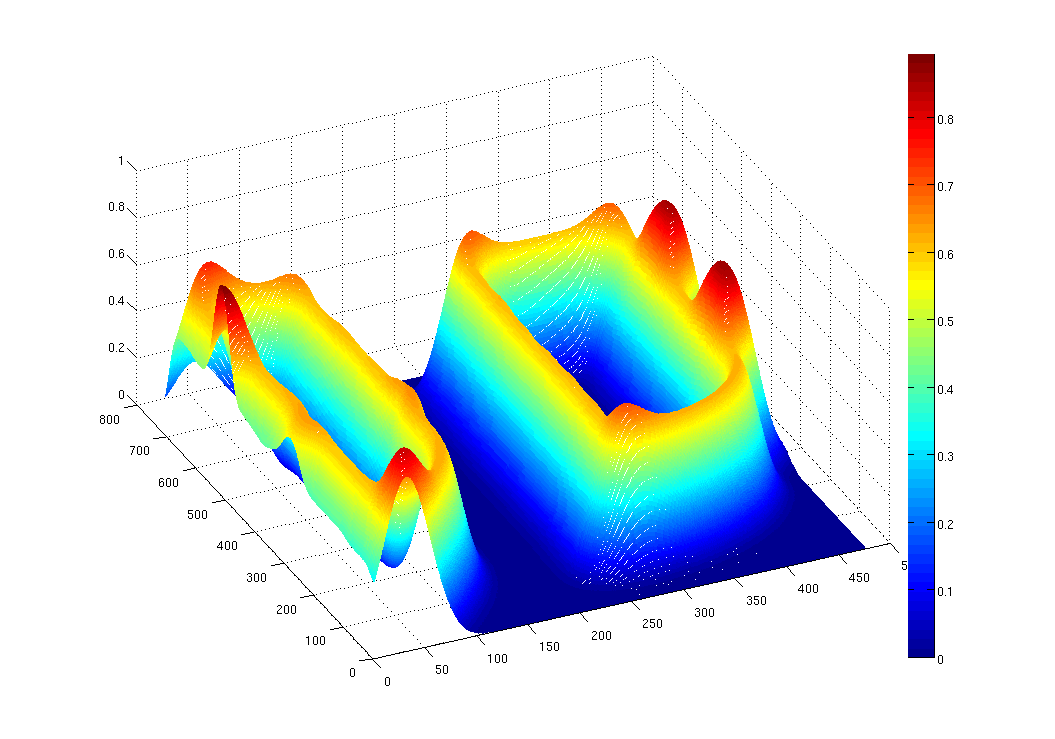
\includegraphics[height=3in]{02_densitymask3D}
    \caption{Colormap demonstrating point densities at different pixel locations}
    \label{fig:02_densitymask3D}
\end{figure}


